

Abychom mohli hovořit o konkrétních technologicích, musíme nejdříve definovat základní stavební technologické kameny, o které se BigData opírají. Jedná se o technologie a paradigmata vyvinutá technologickými giganty, kteří jako první naráželi na technologické hranice a posouvali je dál a tak se postupně rodily tyto technologie a paradigmata. Jejich pořadí se odvýjí od logické posloupnosti tak, jak spolu souvisí a navazují na sebe.    

\section{Distribuované systémy}
Distribuované systémy, jsou tématem, které zasahuje samozřejmě mnohem dále, než jen do kategorie big data. Pro zjednodušení následujících řádků, zavedeme následující rozdělení. Distribuované systémy rozdělíme na systémy s distribuovaným výpočetním výkonem, systémy s distribuovaným úložištěm a nebo kombinace obojího. 

Distribuovaný výpočetní výkon, je takový systém, kde se výpočet jedné úlohy rozloží na více počítačů. Paralelní výpočety jsou známé z oblasti informačních technologií, již mnoho let a používají se nejčastěji k vědeckým výpočtům, paralelní kompilaci zdrojových kódů a nebo k jiným operacím, které by na jednom počítači trvaly příliš dlouho. 

Distribuované úložistě je jednoduše představitelné a důvodů mít data na více místěch je hned několik.
\begin{itemize}
\item Záloha - i ze sféry osobních počítačů známé trend kde máme data zálohovaná na více fyzických zařízeních, abychom předešli jejich ztrátě, v případě technické poruchy na daném zařízení. 

\item Nedostatek kapacity - Ze sféry osobních počítačů známe, že uživatelé, méně potřebné soubory ukládají na externí periferie, protože kapacita disků v osobních počítačích je zpravidla kolem pár TB.

\item Dostupnost - Pokud chce uživatel mít přístup k jednomu souboru z domácího i pracovního počítače, musí soubor mít fyzicky na těchto dvou počítačích, nebo využít nějaký software na sdílení souborů. 

\end{itemize}

Kombinovaný přístup je zřejmy a tedy, že se používá jak výpočetní výkon jednotlivých počítačů v systému, tak jejich úložný prostor. 

Big Data využívá všechny tyto přístupy, je zřejmé že obrovské množství dat, o kterém jsme mluvili v úvodu se lépe zpracovává na více počítačích. Stejně tak je logické, že pokud budeme bavit o množství dat, tak velké množství dat, uložíme na více počítačů, stejně tak pokud data chceme zálohovat. 

Ne vždy však využíváme kombinovaný přístup, je totiž velmi časté, že si firmy staví obrovské počítačové farmy, které slouží pouze jako datové sklady a datová centra. Vždy záleží na konkrétní situaci a způsobu využití. 


\section{CAP Theorem}
V roce 2000 při nástupu distribuovaných systémů vydal vědec Eric Brewer článek, popisucjíí tzv. CAP Theorem \cite{cap}, který se distribuovaných systémů přímo týká. Teorém říká, že distribuované systémy mají tyto 3 hlavní vlastnosti. 

\begin{itemize}
\item Konzistence (Consistency) - Vlastnost, která určuje, zda pro každý požadavek, vratí server správný výsledek. to znamena že odpověd je adekvátní vůči specifikaci požadované služby. Přesný význam konzistence se odvýjí od typu služby. V případě dat ji definujeme tak, že každý server má aktuální a stejná data.

\item Dostupnost (Availability) - Vlastnost která říka, že každý požadavek dostane odpověd. Rychlejší odpověd, je preferovanější oproti pomalejší, ale v kontextu teorému je důležité, že odpověd dorazí. V praxi však znamená, že velice opožděná odpověd je stejně spatná jako žádná odpověd a můžeme tuto vlastnost zjednodušit, že systém vždy musí být dostupný.

\item Tolerance výpadku (Partiotion tolerance) - Tato vlastnost jako jediná určuje chování podpůrného systému na kterém služba běží, namísto popisu chování služby samotné. Tato vlastnost říká, jestli během výpadku nějaké části systému, je systém schopný pokračovat a dále fungovat.

\end{itemize}


Brewer popisuje, že každý distribuovaný systém může splňovat nejvýše 2 z těchto 3 vlastností.

\subsection{CAP Theorem v roce 2012}
V roce 2012 napsal Brewer další článek \cite{cap2}, ve kterém popisuje stav jeho theorému po 12 letech. Vysvětluje, že již od začátku bylo označení \uv{pouze 2 ze 3} zavádějící a vágní, protože spoustu věcí příliš zjednodušovalo. Například u systému s velkou granularitou,  se mezi volbou C a A rozhoduje na několika úrovních a všechny vlastnosti mají spíše hodnoty v čase, než binární a také, že záleží na stavbě systému a jeho drobných nuancích. Také ale píše, že v důsledku theorém splnil svůj účel a otevřel tak systémévým návrhárům oči pri navrhování distribuovaných systémů a donutil je zamyslet se nad vyhodami a nevýhodami jednotlivých vlastnotí systému. 

V témže roce vyšel další zajímavý článek popisující aktuální stav CAP theorému \cite{cap3}. Popisuje převážně vztah
systémů k volbám CAP vlastnostní. 

\subsubsection{Nejlepší možná dostupnost}
Nejčastejší výběr je garantovaná konzistence s maximální možnou dostupností, pro většinu systémů je toto přirozenou volbou. Tedy, že za každou cenu, server vrací správnou odpověd a snaží se poté optimalizovat co největší dostupnost a nejrylechjší možnou odpověd vzhledem k síťovým podmínkám. Tento přístup dává největší smysl pokud jsou počítače ve stejném datacentru a běží na nich stejná služba. Typickým zástupcem je  \uv{lock service} a služba spravující metada pro nějaký distribuovaný systém s nízkou granularitou.

\subsubsection{Nejlepší možná konzistence} 
Druhou nejčastější skupinou jsou systémy, pro které je ztráta dostupnosti nemyslitelná a tudíž garantují dostupnost a snaží se o co nejvyšší úroveň konzistence. Tento postup nejlépe vyhovuje v případech kdy máme počítače distribuované napříč několika datacentry, v tomto případě může totiž dostupnost rapidně klesat s jakoukoliv chybou a proto je potřeba ji garantovat. V těchto případech tedy designéři obětují konzistenci, aby mohli garantovat dostatečně rychlou odpověd, přestože ta nemusí být vždy zcela správná. Ideálním příkladem jsou webové cache a obrázkové servery.

\subsubsection{Segmentovaná konzistence a dostupnost}
toto je nejzajímavější možnost a pro tuto práci je také nejdůležitější. Existují systémy, které nemají jednotné požadavky pro všechny aspekty služby. Některé vyžadují silnou konzistenci a některé vysokou dostupnost. Pro dodžení CAP theoremu se  jako nejpřirozenější možnost jeví rozdělit systém na několik jednotlivých komponent, které budou specificky nastaveny. tím tedy celý systém nezaručuje ani konzistenci, ani dostupnost, ale každá část systému postkytuje opravdu vlastnosti, které potřebuje. Segmentace může probíhat na několika možných úrovních. 

\begin{itemize}
\item \textbf{Rozdělení podle dat} - jiná data mohou vyžadovat jinou úroveň dostupnosti a konzistence.
\item \textbf{Rozdělení podle operací} - Operace pro zápis mohou mít jiné požadavky na konzistenci a dostupnost, než operace pro čtení.
\item \textbf{Rozdělení podle funkcí} - Některé služby mohou být rozděleny na podslužby a tedy pro každou takovouto službu můžeme mít vlastní úroveň konzistence a dostupnosti. 
\item \textbf{Rozdělení podle uživatelů} - Jedná se o rozdělení závislé převážně na geografické poloze uživatele, služba bude pro uživatele, který se nachází blízko může zaručit vysokou dostupnost a zároveň v rámci jeho blízkého data centra udržovat i konzistenci. 
\item \textbf{Rozdělení podle hierarchie} - Jedná se o systém ve kterém se na určitých úrovních kombinují výše popsané rozdělení.
 
\end{itemize}
\section{Distribuovaný file systém}

V předchozích sekcích jsme rozebrali distribuované systémy a jejich omezení. Zmínili jsme také, nutnost sdílet velké množství dat napříč několika počítači, které můžou být napříč různými datacentry. Tuto potřebu, tedy mít distribuovaný filesystém, měl i jeden z největších technologických gigantů, firma Google. V roce 2004, se Google rozhodl o jejich řešení podělit a vydal detailní článek \cite{gfs} popisující kompletní funkčnost a detaily celé infrasntruktury. Vysvětlení funkčnosti a  architektury je nad rámec této práce a navíc je vše dobře popsané v článku samotném, důelžité je však zmínit, že tento systém se stal inspirací a nastolil trend v tom, jak podobné systémy dnes vypadají a jaké mají vlastnosti. Na základě tohoto článku vznikl například opensource klon MooseFS.

\begin{figure}[h]
\centering
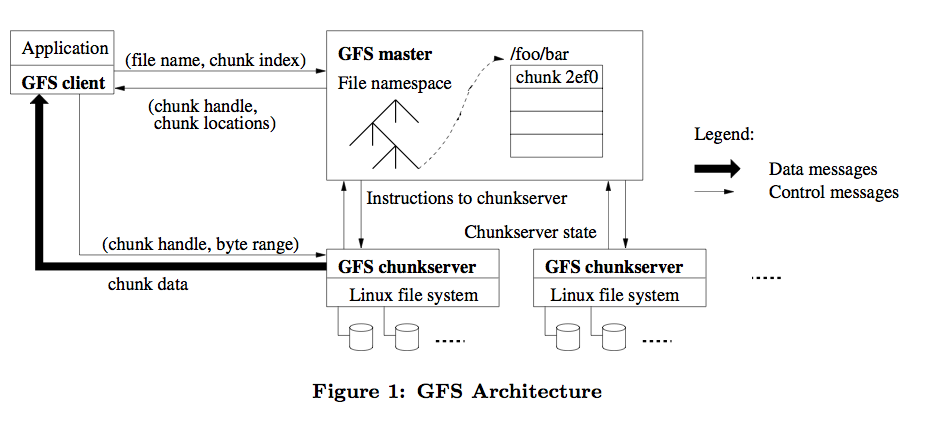
\includegraphics[scale=0.5]{images/gfs}
\caption{Architektura Google File System \cite{gfs}}
\label{fig:3v}
\end{figure}

\section{BigTable}
Jedná se o systém na uchovávání dat spoledčnosti Google, který je postavený nad Google File Systémem a jinými technologiemi společnosti Google. Jedná se o proprietární software, který není kdispozici mimo firmu Google, kromě možnost využívat tento sw jako část služby Google App Engine.  V roce 2006 opět google zveřejnil článek o BigTable \cite{bigtable}, avšak nyní s mnohem méně detaily, nežli u svého článku o GFS \cite{gfs}, kvůli obavám o přesné zkopírování jako u zmíněného systému. V době vydání článku bigtable obsluhoval více než 60 služeb firmy Google a škáloval několik Petabytů dat na několika tisici počítačích. BigTable umožňuje využívání MapReduce frameworku. Jedná se o první implementaci mnoho sloupcové, distribuované, multidimenzionální perzistentní seřazené mapy.  Google opět udal trend jakým se podobné systémy začali ubírat. Datový model BigTable v budoucnu inspiroval i tvůrce Apache Cassandra, která je hlavním tématem této práce a proto detaily ohledně datového modelu prozatím přeskočíme.

\section{MapReduce}
Je programovací model a framework prvně představený společností Google \cite{mapreduce} na zpracování velkého datasetu. Uživatel specifikuje mapovací funkci, která zpracuje páry (klíč, hodnota) a vygeneruje přechodné páry (klíč hodnota), které jsou pak předané redukovací funkci, která sloučí všechny mezi-hodnoty se stejným mezi-klíčem. Mnoho příkladů z reálného světa, lze převézt do tohoto paradigmatu. Výhodou těchto funkcionálně napsaných programů je, že jsou automaticky velice paralelizovatelné. Systém se stará o detaily distribuce dat a rozhození jednotlivých uloh na jednotlivé počítače a obsluhuje chyby a neočekávané stavy. toto umožňuje programátorům i s velice malou znalostí paralelního programování napsat vysoce paralelní a efektivní programy. 

Toto paradigma se stalo v nejdůležitějším stavebním kamenem pro zpracovavání BigData. Díky tomuto mechanizmu jsme schopni zpracovávat Terabyty dat rychle a efektivně a vypočítaný výsledek znovu uložit do databáze. Veškeré postupy zpracování BigData jsou přímo, či nepřímo založené na MapReduce. 

\begin{figure}[!h]
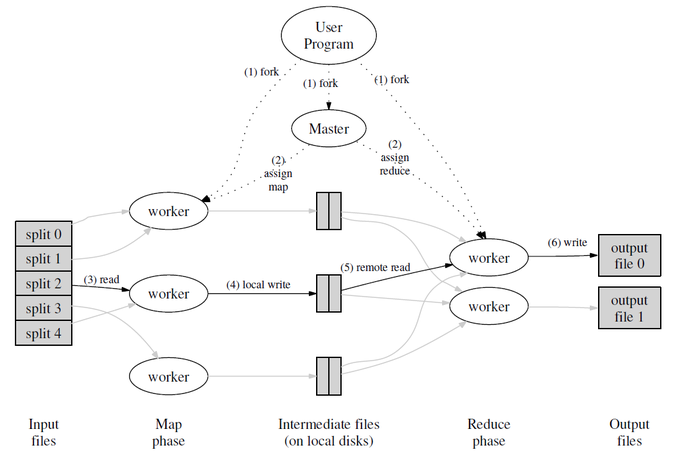
\includegraphics[scale=0.6]{images/mapreduce}
\caption{MapReduce schéma \cite{mapreduce}}
\label{fig:mapreduce}
\end{figure}

\newpage

\section{NoSQL}
Se zkratkou SQL se můžeme u relačních databázových systémů. Zkratka NoSQL neznamená pravý opak, písmena \uv{No} znamenají \uv{Not Only}, tedy ne pouze. Jedná se o databázový koncept, který se vyskytuje u nerelačních databází. V tomto konceptu datové úložiště i zpraování dat používají jiné prostředky, než běžné tabulkové schéma relační databáze. Výhody tohoto konceptu jsou jednoduchá desihn a horizontální i vertikální škálovatelnost. NoSQL databáze často podporují také podmnožinu jazyka SQL a většinou se jedná o jednoduché funkce jako vkládání a velice jednoduché výběry. Některé NoSQL databáze mají i velice odlišný ukládací model, například (stromový, grafový) tím padem je složitost  pro různé operace odlišná. Nejčastější podobu má NoSQL databáze formou klíč hodnota, čili mapa. Podle dosavadních informací lze říci, že Google BigTable je tedy NoSQL databáze. Mezi charakteristiky NoSQL databází můžeme zahrnout

\begin{itemize}
\item \textbf{Datový a dotazovací model} - jak již bylo řečeno NoSQL databáze se liší způsobem udržování dat a  dotazováním nad nimi
\item \textbf{Perzistence} - Ne všechny NoSQL datbáze ukládají svá data na disk, některé databáze běží pouze v operační paměti.
\item \textbf{Rozhraní} - Některé databáze komunikují skrze REST rozhraní a některé pomocí binárních protokolů 
\item \textbf{BASE} - Tak jako relační databáze využívají vlastnosti ACID (Atomic Consistent Isolation Durability) tak v NoSQL je ekvivalentem BASE (Basically Available, Soft state, Eventual consistency) kde každá NoSQL databáze garantuje jednotlivé vlastnosti různými mechanizmy a nastaveními nebo jsou již od základu navržené s danými vlastnostmi.   
\end{itemize}


NoSQL databáze jsou dalším základním stavebním kamenem BigData. NoSQL databáze jsou často kompatibilní s MapReduce konceptem, čímž tvoří ideální dvojici pro uchovávání a zpracování velkého množství dat. 

